\documentclass[dvipdfmx,autodetect-engine,titlepage]{jsarticle}
\usepackage[dvipdfm]{graphicx}
\usepackage{ascmac}
\usepackage{fancybox}
\usepackage{listings}
\usepackage{plistings}
\usepackage{itembkbx}
\usepackage{amsmath}
\usepackage{amssymb}
\usepackage{amsfonts}
\usepackage{svg}
\usepackage{url}
\usepackage{graphics}
\usepackage{multirow}
\usepackage{listings,jvlisting}

\textheight=23cm
\renewcommand{\figurename}{図}
\renewcommand{\tablename}{表}
\newenvironment{code}
{\vspace{0.5zw}\VerbatimEnvironment  
\begin{screen} 
\baselineskip=1.0\normalbaselineskip
 \begin{Verbatim}}
{\end{Verbatim}
\baselineskip=\normalbaselineskip
 \end{screen}\vspace{0.5zw}} 

\title{情報理工学部 SNコース 3回\\
第4回レポート}
\author{2600200443-6\\Yamashita Kyohei\\山下 恭平}
\date{Jan 22 2023}

\begin{document}

\maketitle

\section{問1:既習手法の技術マップ}

\begin{enumerate}
  \item 重回帰分析
  \item 判別分析
  \item 主成分分析
  \item 多次元尺度法
  \item 数量化I類
  \item 数量II類
  \item 数量化IV類
\end{enumerate}

\section{問2:主成分分析}

この課題ではpythonライブラリのscikit-learnで分析を行い,その結果を
matplotlibを用いてプロットした.

\subsection{第2主成分までで2次元平面にプロットせよ}

\begin{figure}[h]
  \centering
  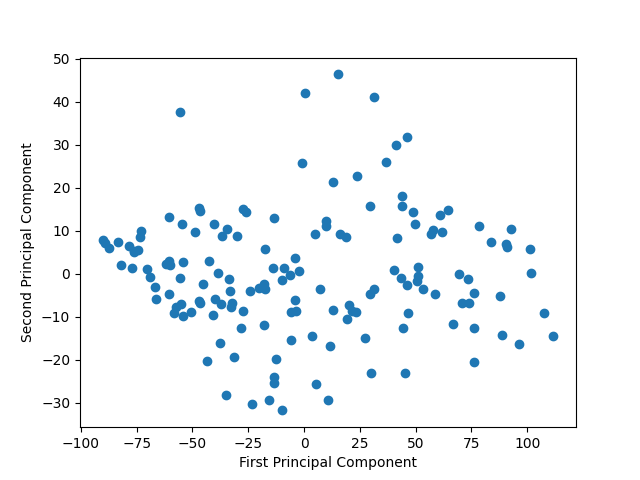
\includegraphics[scale=0.7]{Figure_1.png}
  \caption{第2主成分までのデータ}
\end{figure}

\newpage

\subsection{第6主成分までの累積寄与率をグラフに示せ}

\begin{figure}[h]
  \centering
  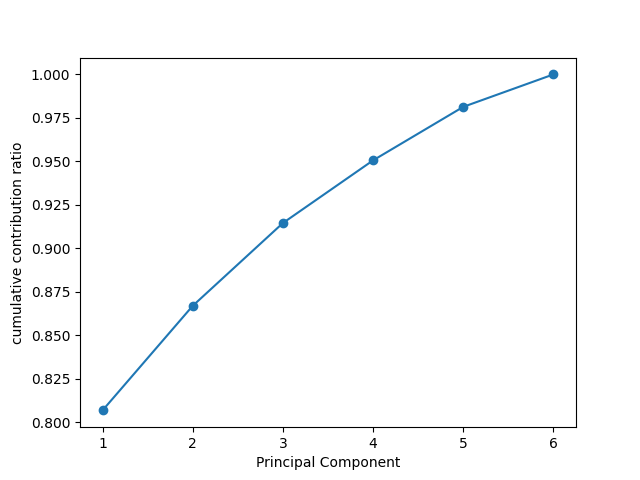
\includegraphics[scale=0.7]{Figure_2.png}
  \caption{第6主成分までの累積寄与率}
\end{figure}

\subsection{6つの主成分について, 6項目の特徴の主成分負荷量を求め,各種成分がど のような意味をもつのかを解釈せよ.}

6つの主成分における6項目の主成分負荷量は以下のようになる

\begin{figure}[h]
  \centering
  \fbox{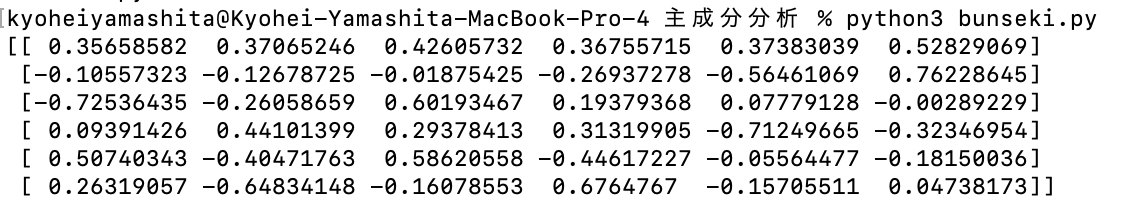
\includegraphics[scale=0.7]{Figure_3.png}}
  \caption{6項目の特徴の主成分負荷量}
\end{figure}

第一主成分については,6項目全てが近い値をとっており,全て正であることから,点数
が上がれば上がるほど\begin{math}y_1\end{math}は大きくなる.\\
第二主成分は「博士過程学生の多さ」意外全てがマイナスであることから,博士過程学生の多さに
ついての因子であると考えられる.\\
第三主成分からは学生が多く,女子学生の比率が高い時\begin{math}y_3\end{math}の値が大きくなることが分かる.\\
第四主成分は教室の広さについて因子だと考えられる.\\
第五主成分は図書館蔵書と女子学生の比率が高い時\begin{math}y_5\end{math}が大きくなる\\
第六主成分は教員の多さについての因子である.

\end{document}